\phantomsection

\chapter{\uppercase{MULTIMODAL CONTEXTUAL DIALOG BREAKDOWN DETECTION FOR CONVERSATIONAL AI MODELS}}


\section{Phone Call Dialog Breakdown Examples}
\label{sec:db_example}

Different from dialog breakdown examples from interactions between users and text-only chatbot AI agents, conversation flows of dialog breakdown from our phone call data contain various types of examples with a higher complexity caused by additional factors such as audio-related issues, real-time conversation latency expectations, and health insurance benefit verification standard operation procedures. For example, users can take various lengths of pause between their utterances while they provide long sequences of information (e.g., phone numbers, patient ID, processor control number or bank identification number) so AI agents may confuse short pauses of users in the middle of the full sequence with an end of speech and start asking next questions (Figure~\ref{fig:dialogue_breakdown_example1_ai_agent_interruption}). The variance of speech pace and lengths of pauses from users can confuse AI agents and aggravate the situation even further when the user's speech contains multiple confusing utterances in a row due to potentially various underlying factors, such as incorrect ASR finalization, which may cause intent misclassification in the downstream pipeline of AI agents (Figure~\ref{fig:dialogue_breakdown_example1_ai_agent_goes_silent}). More complex examples include more subtle, nuanced situations in which AI agents apparently drove conversations correctly but missed required actions, which may lead to call failure in the later phase of the call (Figure~\ref{fig:dialogue_breakdown_example1_ai_agent_skipping_actions}).

\begin{figure}
    \centering
    \small
    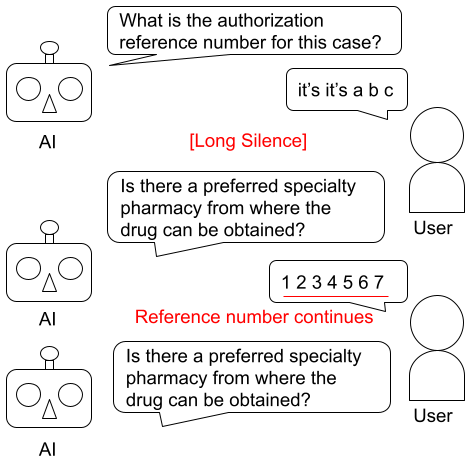
\includegraphics[width=3in]{images/db_Dialogue Breakdown Example 1 Eva Interrupting Agents.png}
    \caption{AI Agent misunderstood a partial sequence `abc' followed by a relatively long pause from the user as a full reference number and interrupted the user by asking its next question in the middle of the user speech.
    }
    \label{fig:dialogue_breakdown_example1_ai_agent_interruption}
\end{figure}



\begin{figure}
    \centering
    \small
    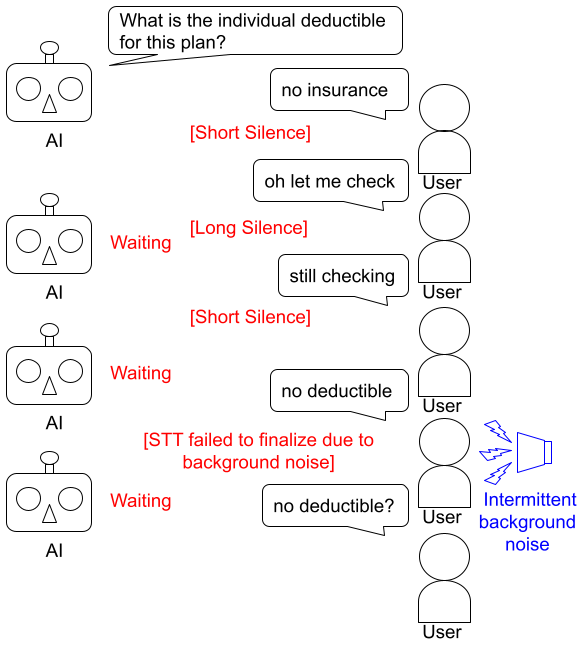
\includegraphics[width=3in]{images/db_Dialogue Breakdown Example 3 Eva went silent.png}
    \caption{AI Agent went silent even when the user provided an answer due to the combined factors of ASR STT finalization, downstream intent misclassification.}
    \label{fig:dialogue_breakdown_example1_ai_agent_goes_silent}
\end{figure}





\begin{figure}
    \centering
    \small
    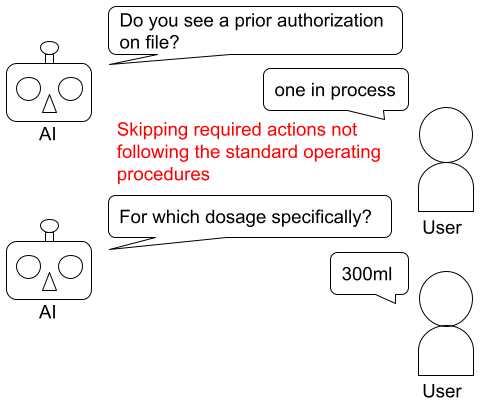
\includegraphics[width=3in]{images/db_Dialogue Breakdown Example 2 Eva skipped actions.png}
    \caption{AI Agent should have asked if there is an active prior authorization which can cover target medication when the user said `one in process' instead of proceeding with the pending prior authorization asking its next question.}
    \label{fig:dialogue_breakdown_example1_ai_agent_skipping_actions}
\end{figure}



\section{Preliminary Analysis}
\label{sec:prelim}
We conducted preliminary analysis using the latest state-of-the-art conversational AI models to validate the task, dataset and level of difficulty for dialogue breakdown model development.

\subsection{Gemini Pro In-Context Learning}

We used in-context learning (ICL) approaches with Gemini Pro as this model did not support fine-tuning and selected Gemini over other LLM vendors due to the status of security review at the time to remain HIPAA compliant. We provided randomly selected N calls from training set with the prompt in the format presented below. 

The largest number of sample calls were used as examples in context as long as Gemini Pro context limit allows (32,000 tokens); prompts with 33 call or more examples caused `invalid argument' errors based on the lengths of sampled calls. We used temprature = 0, top\_p=1, top\_k=40, candidate\_count=1 and max\_output\_tokens=8000. We conducted random sampling for ICL call examples with random seed of default value (None) and from 0 to 9 and reported mean, 25\% and 74\% percentile F1 performances of 11 iterations of each number of example calls. The highest mean F1 score of Gemini Pro PCL was 40.31 when it had 31 random example calls and this number was reported in our main paper (Section~\ref{sec:task_eval}).

\begin{tcolorbox}[title={Prompt}]
Given a conversation between an AI agent and a user, find a dialog breakdown turn which may need a human intervention.

The conversation is in the following format:

"(turn number) [AI Agent]: \textit{AI utterance} | (turn number) [User]: \textit{user utterance}".

Return which turn needs human intervention due to dialog breakdown. 
For example, from the conversation input 

"(1) [User]: How are you today | (2) [AI Agent]:I want to eat ice cream", 

You can return 2 because the second turn was off-topic.

Which turn do you think may cause a dialog breakdown, so it may need some human intervention in the following conversation?

Here are some real phone call conversation examples:

\{ Example N calls randomly selected from training set in the given conversation format along with their ground truth breakdown turns \}

Now, provide your answer from this conversation:

\{Testset call in the given conversation format\}
\end{tcolorbox}

The general trend of F1 score was increasing up to this point with a few decreasing patterns in the middle and this general trend aligns well with the findings from related prior work~\cite{Zhao2021CalibrateBU,liu-etal-2022-makes,min2022rethinking}. However, Gemini does not have explicitly encoded information for the healthcare industry phone calls from our datasets so its performance tend to fluctuate based on which calls are sampled as context examples for detecting dialog breakdowns from the given test calls.

\begin{figure*}
    \centering 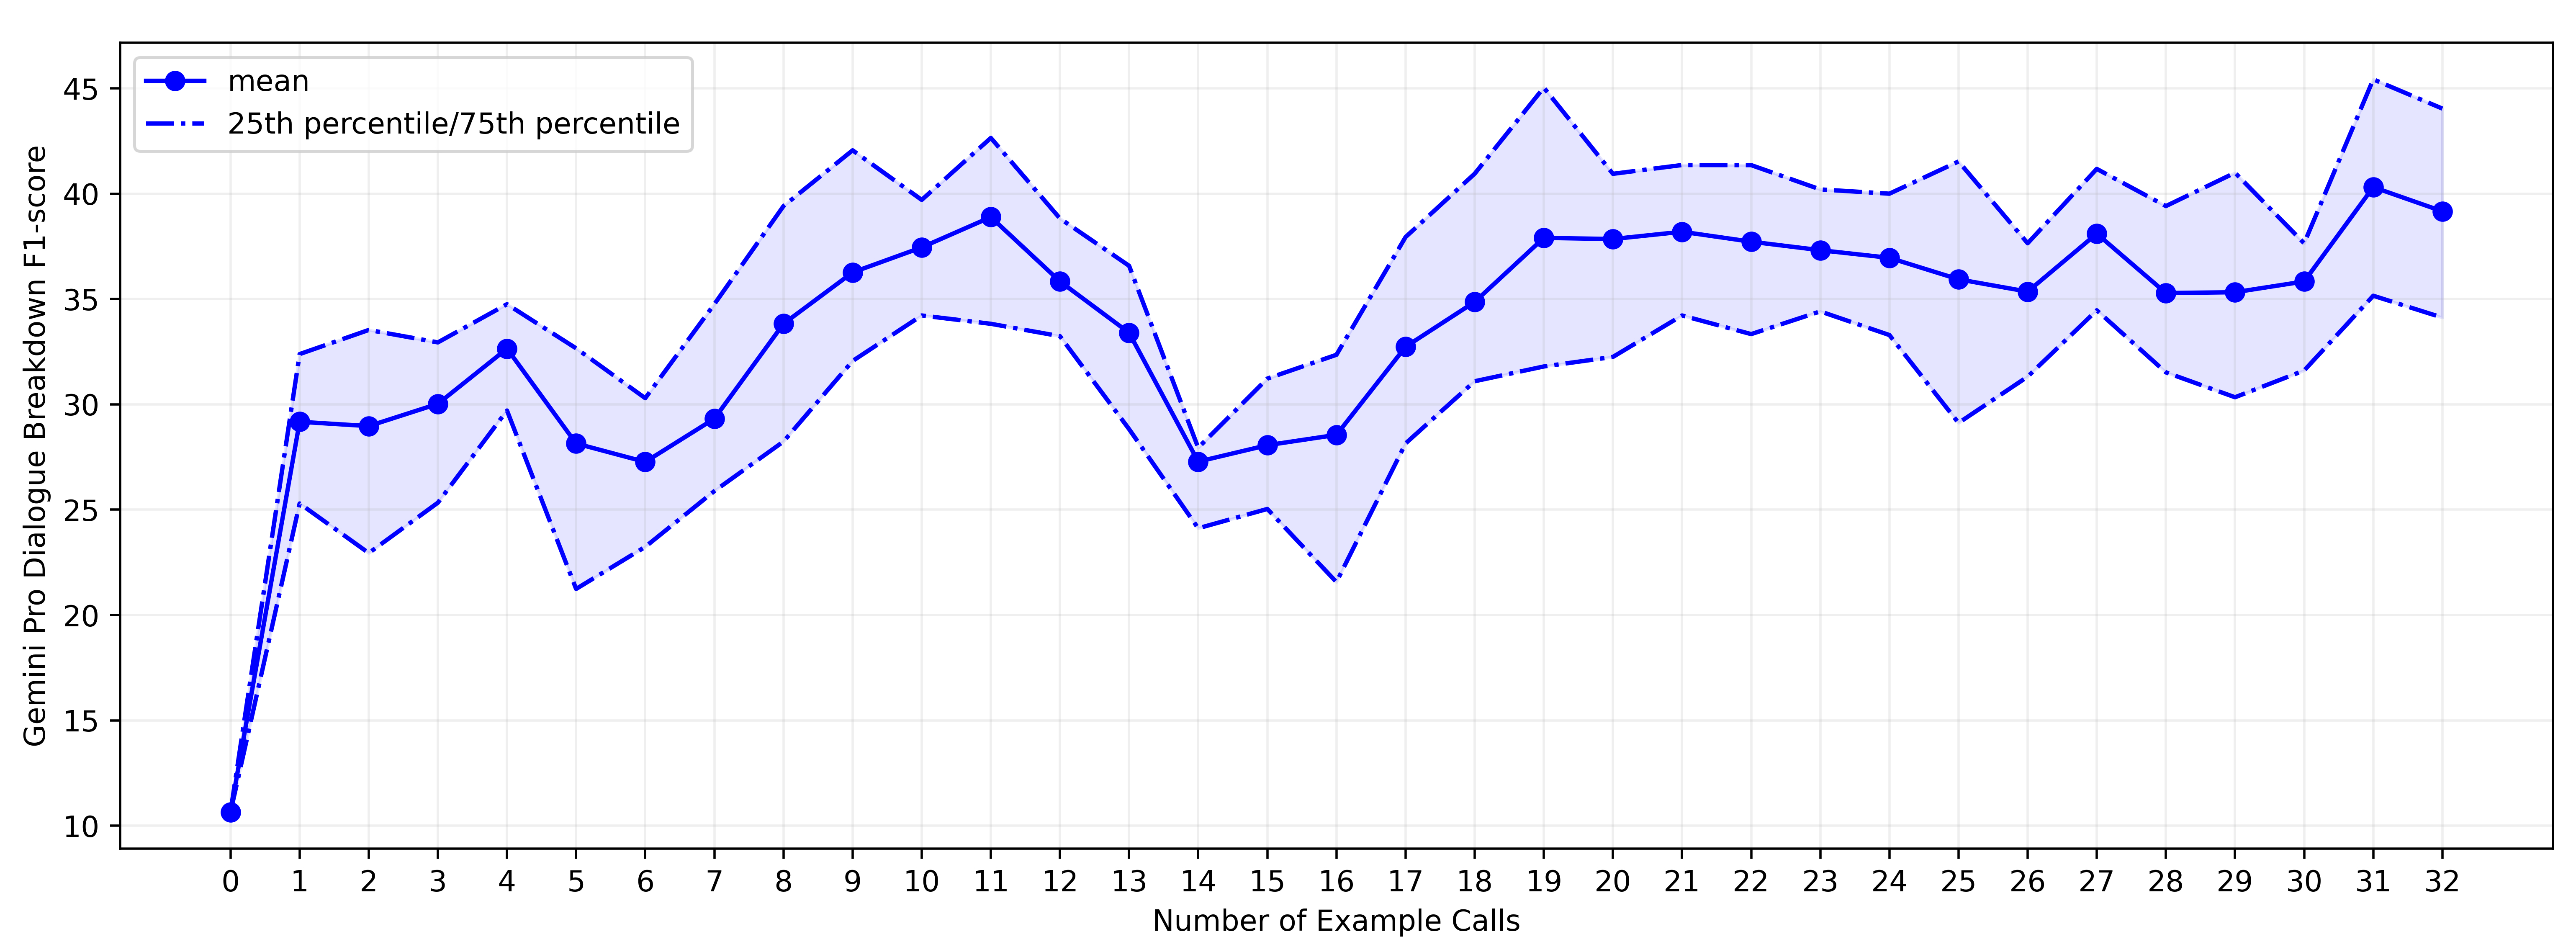
\includegraphics[width=6in]{images/db_F1_score_gemini_ICL_32_iter_10_random_seeds_one_legend_cropped.jpg}
    \caption{Gemini Pro in-context learning dialogue breakdown prediction performance changes among the number of example calls provided in context.}
    \label{fig:gemini_pro_ICL}
\end{figure*}


\section{Model and System configurations}
\label{sec:model_config}
\subsection{Text LSTM}
\label{sec:model_config:text_lstm}
\textbf{Input Processing:} Each utterance is represented in the format -  `speaker: \textit{speaker tag (AI agent or user)} | utterance: \textit{utterance text generated by ASR} | intent: \textit{intent of the utterance from AI Agent input classification model}' and passed as the input to the feature extractor model.
\subsection{End-to-End LLM}
\label{sec:model_config:e2e_llm}
\textbf{Input Processing:} Each input to the model is represented in the format - `<s> \textit{current utterance representation} </s> \textit{four previous utterance representations} </s>.' Then we join the current utterance representation and the four previous context utterance representations with the separator token. The input is passed to the RoBERTa-base model, and we extract the embedding of the sentence start token, <s> as the utterance embedding and pass it to a set of linear layers for classification.
\subsection{MulT A+T}
\label{sec:model_config:mult_at}
\textbf{Input Processing:} Specifically, we employ RoBERTa as the textual feature extractor, following a similar process as described in \ref{lstm} to extract token embeddings. For acoustic features, we utilize Wav2Vec2 \cite{10.5555/3495724.3496768} to extract information from the raw waveform data. To ensure consistency, we pad or trim every utterance signal to a fixed duration of 15.0 seconds. After extracting the modality-specific features, we apply two 1D convolutional layers, each consisting of 256 kernels with a size of 5, to make the input features aware of their temporal neighborhood.
\subsection{MultConDB} \label{sec:model_config:multcondb}

\textbf{Hyperparameters:} To ensure the reliability of the results, each experiment is carried out using three different seeds. The primary metric for evaluating the results is the F1 score. The training process continue for 40 epochs, with an early-stopping mechanism implemented to stop training if there is no improvement in the F1 score for five consecutive epochs. Table \ref{tab:hyperparameters} displays a detailed list of hyperparameters along with the values selected based on experimentation.


\begin{table}
\small
\centering
\begin{tabular}{|l|l|}
\hline
\textbf{Name} & \textbf{Best Value} \\
\hline
Batch size & 32\\
Hidden dimensions of encoders & 128\\ 
Kernel size of conv layers & 5\\
No of channels of conv layers & 256\\
Window size for context modeling & 5\\
\hline
\end{tabular}
\caption{Choice of hyperparameters}
\label{tab:hyperparameters}
\end{table}

\textbf{Design Choices:} In our implementation, we use Wav2vec2 as the acoustic feature extractor instead of Whisper which is used as a feature extractor in \cite{miah-etal-2023-hierarchical}. However, Whisper \cite{radford2023robust} requires audio chunks to be adjusted to a fixed length of 30 seconds, which significantly exceeds the typical duration of utterances in our dataset. Wav2Vec2 offers flexibility in terms of audio chunk length, allowing us to use 15 second chunks. This not only makes our model more memory-efficient but also speeds up the inference process to meet the demands of our online task. To improve the model's online performance, we opt to restrict the context size to 5. Through experimentation with various context lengths during inference, we observe that while a larger context typically yields better performance, it also increases the inference time. In our design, we use a context length of 5, which strikes a balance between achieving satisfactory performance and maintaining fast inference speed. The inference time is 0.06s for each utterance.